\documentclass[11pt,a4paper]{article}
\usepackage[utf8]{inputenc}
\usepackage[T1]{fontenc}
\usepackage[polish]{babel}
\usepackage{lmodern}
\usepackage{graphicx}
\usepackage{epstopdf}
\usepackage{anysize}
\usepackage{makeidx}



%\def\projectsymbol
\makeatletter
\renewcommand{\maketitle}{
\begin{titlepage}
\begin{center}

\LARGE{AKADEMIA GÓRNICZO-HUTNICZA}

\vspace*{1cm}

\includegraphics[scale=1.8]{agh.eps}
\vspace*{1cm}

\LARGE{im. Stanisława Staszica w Krakowie}

\rule{\textwidth}{0.4mm}
\LARGE \textsc{\@title}
\rule{\textwidth}{0.4mm}

\vspace*{5mm}
\begin{flushright}

    \begin{minipage}{5cm}

    \textit{\small Autorzy:}\\
    \normalsize \textsc{\@author} \par

    \end{minipage}

\end{flushright}
\vspace*{\stretch{8}}
\rule{\textwidth}{0.4mm}

\large{Wydział Elektroniki, Automatyki, Informatyki i Elektrotechniki}\\
\large{Katedra Automatyki}\\
\large{Laboratorium Biocybernetyki}\\
\vspace*{\stretch{7}}
\@date

\end{center}

\end{titlepage}
}
\makeatother

\title{Lokalizacja twarzy na obrazie za pomocą konwolucyjnych sieci neuronowych}
\author{Bartłomiej Bułat\\
    Tomasz Czarnik\\
    Krzysztof Śmiłek\\\\}
\date{\today}

\makeindex

\begin{document}

\maketitle
\printindex


%=================================================
\section{Streszczenie}

Celem naszego projektu jest zbudowanie prototypu systemu pozwalającego na detekcję twarzy na obrazie 
w oparciu o sieć neuronową typu CNN (Convolutional Neural Network).
%=================================================
\section{Wstęp}

\subsection{Co to jest sieć neuronowa?}
Siec neuronowa jest modelem matematycznym składającym się z sieci węzłów obliczeniowych zwanych neuronami
 i ich połączeń. Jest to pewna technika obliczeniowo-statystyczna, należąca do dziedziny sztucznej inteligencji. 
Jej zadaniem jest symulacja działania ludzkiego mózgu. 

\subsection{Budowa sieci neuronowej }
Nasz mózg jest zbudowany z ogromnej ilości neuronów które komunikują się ze sobą za pomocą impulsów elektrycznych.
 Z informatycznego punktu widzenia neuron stanowi układ przetwarzający pewne dane, posiadający wiele wejść
 oraz jedno wyjście. Oto porównanie neuronu naturalnego ze sztucznym:

\vspace*{1cm}
\hspace*{1cm}
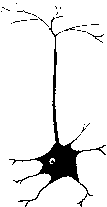
\includegraphics[scale=0.7]{neuron}
\hspace*{1cm}
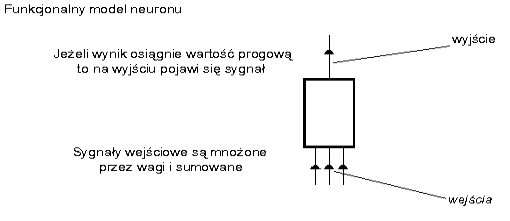
\includegraphics[scale=0.7]{neuron2}
\hspace*{1cm}
\vspace*{1cm}

Działanie sztucznego neuronu można opisać w przybliżeniu następująco:\\
Sygnały $x_{i}$ podane na wejścia są mnożone prze odpowiednie wagi $w_{i}$ oraz sumowane.
 Wagi mogą przyjmować dowolne wartości rzeczywiste. Równanie neuronu wygląda zatem następująco:
\begin{center}
$Y = x_{1}w_{1} + x_{2}w_{2} + x_{3}w_{3} + … + x_{n}w_{n} + b$\\
\end{center}
Suma ta staje się następnie argumentem funkcji aktywacji, która zwraca wartości z zakresu 
(-1,1). Wynik tej funkcji pojawia się zarazem na wyjściu z neuronu.\\
\\
Jak zapewne możemy zauważyć pojemność pojedynczego neuronu nie jest duza, a więc nie może on zapamiętać 
zbyt dużej ilości wzorców. Aby tego dokonać należy połączyć wiele pojedynczych neuronów w sieć. 
Dokonuje się tego tworząc kolejne warstwy. Czym więcej warstw tym sieć bardziej złożona.
 Ilość neuronów w poszczególnych warstwach może się różnić i zależy od konkretnego zastosowania sieci.
 Należy do tego dodać, że neurony w jednej warstwie nie są połączone ze sobą, natomiast neurony z dwóch
 sąsiednich warstw są połączone "każdy z każdym". Sygnał przechodzi do warstwy wejściowej poprzez ukrytą 
aż do wyjściowej, skąd jest odbierany i interpretowany.
%=================================================
\section{Proponowane rozwiązanie}
\subsection{Konwolucyjne znajdowanie twarzy}
\vspace*{1cm}
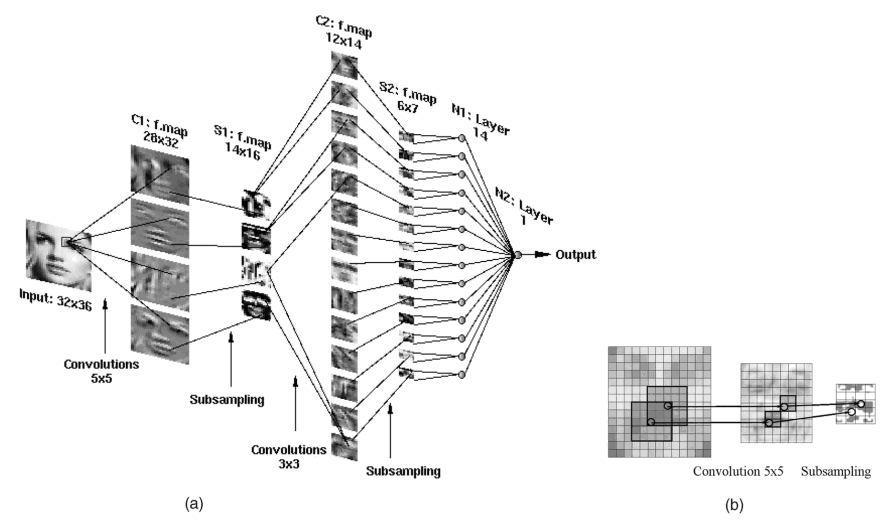
\includegraphics[scale=0.7]{schemat}
\vspace*{1cm}

Sieć ta składa się z sześciu warstw. Do warstw nie wlicza się obraz wejściowy o rozmiarach 32x36,
który będzie klasyfikowany jako „twarz” lub „nie-twarz”. \\
\indent 
Warstwy od \textbf {C1} do \textbf{S2} składają się z serii obrazów na których są przeprowadzane operacje konwolucji lub subsamplingu.
 Obrazy te są nazywane inaczej mapami cech, ponieważ każdy z nich wydobywa z obrazu wejściowego inną cechę. 
Warstwa  \textbf{N1} zawiera szereg niezależnych od siebie neuronów podłączonych wyjściami do  \textbf{N2}, 
która jest zarazem zakończeniem całej sieci neuronowej. Każdy element w danej warstwie otrzymuje 
na wejście informacje od małego zbioru elementów z warstwy poprzedniej. Koncepcję te pokazano na rysunku  \textbf{(b)}.\\
\indent 
Postaramy się teraz opisać dokładniej poszczególne elementy tworzące  przedstawioną powyżej architekturę 
sieci neuronowej. Różne parametry opisujące całą sieć tj. ilość warstw, ilość elementów w warstwie,
 rodzaj połączeń między nimi a także wielkość poszczególnych elementów została wybrana doświadczalnie przez C. 
Garcia i  M. Delakis. Przetestowali oni szeroki zakres wielu architektur sieci i przedstawiona powyżej okazała się
 najbardziej skuteczna zarówno pod względem wykrywalności twarzy jak i odporności na zakłócenia obrazu.\\
\indent 
Warstwa  \textbf {C1} jest złożona z czterech map cech. Rozmiar każdej z nich to 28x32 pikseli. 
Każdy piksel w każdej mapie jest połączony z 5x5 sąsiedztwem z obrazu wejściowego i jego wartość odpowiada
 sumie ważonej tego sąsiedztwa (5x5). Dodatkowo do sumy tej jest dodawana dodatkowa zmienna trenowana
 zwana biasem. Podsumowując, w warstwie tej znajduje się 106(4x26) trenowanych zmiennych.\\
\indent 
Warstwa  \textbf{S1} złożona jest z czterech map cech. Każda z map powstała poprzez subsampling mapy 
z poprzedniej warstwy z maska 2x2, przez co jej rozmiar to połowa rozmiatu poprzedniego. Z każdych 
4 sąsiednich pikseli maski \textbf{C1} jest brana średnia, która jest nastepnie mnożona przez trenowalna zmienną.
Do otrzymanej wartości dodawany jest bias, po czym wynik staje się argumentem do funkcji aktywacji 
(tangensa hiperbolicznego). Funkcja ta używana jest po to, by uniknąć wykroczenia poza zakres zmiennych.
Podsumowując, warstwa  \textbf{S1} składa się z 4 map cech o rozmiarze 14x16 oraz 8(4x2) trenowalnych parametrów.\\
\indent
Jak mozna zauważyć na rysunku  \textbf{(a)}, kolejne warstwy składają się z coraz większej ilości map cech, ale za to
ich rozdzielczość się zmniejsza. Taki rodzaj systemu sieci został zaproponowany przez Hubela i Weisela i dobrze 
wyodrębnia on z obrazu cechy potrzebne do poźniejszego przetwarzania przez neurony.\\
\indent
Warstwa  \textbf{C2} to konwolucyjna warstwa z 14 mapami cech. Pierwsze 8 powstało w wyniku konwolucji 
z maską 3x3 map z poprzedniej warstwy (każda mapa z  \textbf{S1} produkuje 2 wyjścia).
Pozostałe 6 to złożenia dwóch z czterech map z  \textbf{S1} ($4\choose 2$ $=6$ kombinacji).\\
Oto schemat przykladowego zlożenia map o numerach 1 i 4:\\
\begin{center}
$Y = maska1_{3x3}*mapa_{1}+maska2_{3x3}*mapa_{2}+bias$
\end{center}
Podsumowując, warstwa ta sklada się z 14 map cech o rozmiarze 12x14 pikseli każda oraz z 196(8x(3x3+1)
+ 6x(2x3x3+1)) trenowalnych zmiennych.\\
\indent
Warstwa  \textbf{S2} to warstwa subsamplingu analogiczna do warstwy  \textbf{S1}. 
Zmienia sie tylko ilośc i rozmiar map cech. 
Dostajemy zatem: 14 map o rozmiarach 6x7 oraz 28(14x2) trenowalnych zmiennych.\\
\indent
Ostatnie 2 warstwy składaja sie juz z neuronów. Ich zadaniem nie jest ekstrakcja cech jak miało to miejsce 
w poprzednich warstwach, ale ich klasyfikacja. W  \textbf{N1} każdy z pojedynczych neuronów jest w pełni
połączony z wszystkimi pikselami tylko jednej odpowiadającej mu mapy cech z  \textbf{S2}.
Natomiast w warstwie  \textbf{N2} istnieje tylko jeden neuron, który łączy się z wyjściami ze wszystkich neuronów 
z  \textbf{N1}. \\
\indent
Wszystkie neurony z warstw  \textbf{N1} i  \textbf{N2} wykonują klasyczny iloczyn skalarny pomiedzy wektorem 
wejściowym a wektorem wag, do czego później dodawany jest jeszcze bias. Powstała ważona suma jest nastepnie 
przepuszczana przez funkcję tangensa hiperbolicznego, po to,by wyjście z neuronu stanowila liczba z zakresu $(-1,1).$\\
Wyjście z ostatniej warstwy  \textbf{N2} jest używana do klasyfikacji obrazu jako twarz (result>0) lub nie-twarz (result<0).
Warstwy  \textbf{N1} i  \textbf{N2} mają zatem odpowiednio 602(14x43) i 15 trenowalnych zmiennych.\\

\subsection{Trenowanie sieci}
\indent
Stworzyliśmy zestaw szkoleniowy wybierając ponad 800 obrazków zawierających twarze i nie-twarze. 
Zdjęcia pozyskaliśmy przeważnie z internetowych baz danych ktore udostepniały twarze w różnych perspektywach.
Naszym zadaniem bylo ich wyselekcjonowanie i odpowiednie przycięcie, tak by do sieci neuronowej wprowadzić 
jasno i czytelnie które zdjęcia powinien zakwalifikować jako twarz, a które nie. Zdjęcia staralismy sie takze dobierać w ten
sposób aby skutycznie wyłapać różne cechy na obrazach, tak aby nasz system stał się jak najbardziej niezawodny i aby 
wykrywał twarze z jak największą skutecznościa.\\
\indent
Sam proces przycinania obrazków polegał na tym, aby obrazek przeskalować, bądź przyciąc do wielkości 32x36px. Przy czym
głownym celem było to, aby usta i oczy wybanych osób znajdowały sie na każdym obrazie mniej więcej w tym samym miejscu.
Odległość pomiędzy ustami a oczami jest bowiem znacząca, ponieważ pozwala ona na zachowanie odpowiednich proporcji twarzy.
Proporcje te to : odległość między oczami (około 16px), a między oczami i ustami (18px).\\
\indent
Zbieranie zbioru nie-twarzy okazało się o wiele trudniejsze niż sądziliśmy. Praktycznie każdy obraz nie zawierający twarzy
mógłby posłużyc jako obraz testowy. Jednak w tym wypadku proces testowania jest mniej dokladny. Większą dokladnośc
uzyskuje się podczas testowania obrazków które nie są twarzami, ale je znacząco przypominają. Jednak taki zbiór obrazów
jest z oczywistych względów bardzo trudny do pozyskania, przez co posłużyliśmy sie do testów obrazami losowo wyciętymi
z większych zdjęć przedstawiających krajobrazy. \\\\
\indent
Sam proces trenowania przedstawia się natomiast w następujących krokach:
 \begin{enumerate}
\item Stworzenie zbioru 400 obrazów przedstawiających twarz i 400 nie zawierających jej.
\item Ustawienie zmiennych: BootsIter = 0
\item Wybranie spośród zbioru utworzonego w (1) twarzy po 300 obrazów z twarzą i 300 bez.
\item Trenowanie sieci przez około 10 trenowalnych epok. W każdej epoce używana jest taka sama liczba pozytywnych
i negatywnych przykładów. Trenowanie odbywa się natomiast metodą wstecznej propagacji błędów ze współczynnikiem uczenia
(od 0.005)
\item Inkrementacja zmiennej BootsIter = BootsIter+1;
\item Jeśli BootsIter < 6 to idź do (3)
\item Trenowanie sieci przez kolejne 10 epok, ale już dla całego zbioru obazów.
 \end{enumerate}

Przedstawiony wyżej algorytm został dokladniej opisany w artykule [1]. 
Do końca nie udało nam się go w pelni zrozumieć (dlaczego akurat taka a nie inna liczba iteracji itd), 
jednakże ufamy w pełni jego twórcom.

\subsection{Testowanie}
Proces testowania rozpoczęliśmy wykonując wcześniej wspomniany algorytm krok po kroku. Jednakże podczas nauki 
za pomocą metody wstecznej propagacji błędów zauważyliśmy, że nauka ta nie przynosi żadnych rezultatów.\\
\indent
Po konsultacji z prowadzacym doszliśmy wszyscy do wniosku, że wina najprawdopobobniej leży w tym, 
że twarz jest sama w sobie jest dosyć skomplikowanym obiektem, o mnóstwie cech.
Postanowiliśmy zatem, że zamiast wykrywać twarze będziemy wykrywać na obrazach cyfry, które są prostsze do opisania,
ponieważ posiadają mniejszą liczbę własności.
Ponownie zatem stworzyliśmy bazę obrazów z cyframi i wykonaliśmy wspomniany algorytm dla nowych danych.
Jak sie okazało rezultaty były zaskakujące. Dla tej samej budowy sieci program zaczął rozróżniać cyfry.

Wykres uczenia się systemu dla przeprowadonych testów prezentuje się następująco:

\vspace*{0.5cm}
\hspace*{3cm}
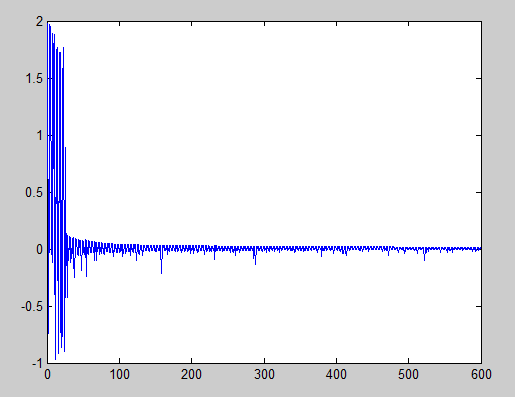
\includegraphics[scale=0.6]{wykres}
\hspace*{3cm}
\vspace*{0.5cm}

Jak możemy zauważyć, z każdą przeprowadzoną iteracją wartość błędu obliczeń się zmniejsza, 
co symbolizuje że sieć uczy się prawidlowo.\\
Tak wyuczoną siec można juz poddać głębszym testom. Postanowilismy tego dokonać tworząc obraz testowy:

\hspace*{4cm}
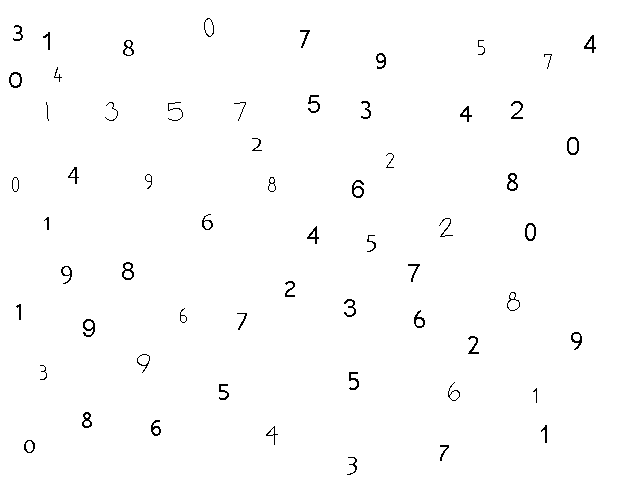
\includegraphics[scale=0.4]{test1}
\hspace*{3cm}
\vspace*{0.5cm}

Po przeprowadzeniu testu otrzymaliśmy zadowalający obraz wynikowy, który potwierdza, że stworzona przez nas 
sieć neuronowa dziala i nadaje sie do wykrywania prostych obiektów np liczb.
Oto otrzymany obraz wynikowy:

\vspace*{0.5cm}
\hspace*{4cm}
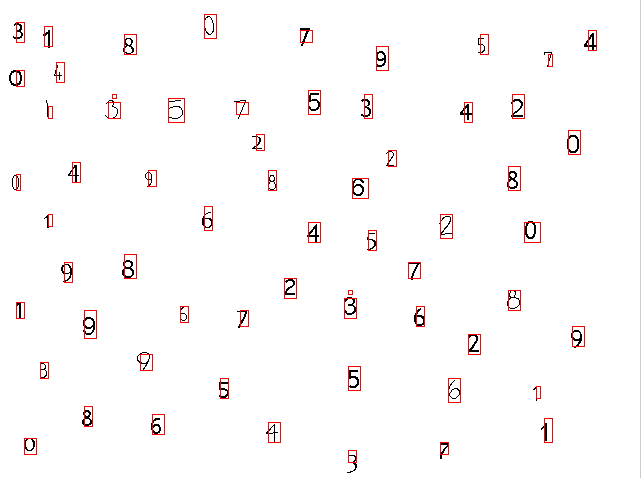
\includegraphics[scale=0.4]{wynik}
\hspace*{3cm}
\vspace*{0,5cm}

%=================================================
\section{Rezultaty i wnioski}

%=================================================
\section{Podsumowanie}

%=================================================
\section{Literatura}
 \begin{enumerate}
\item Convolutional Face Finder: A Neural Architecture for Fast and Robust Face Detection, Christophe Garcia and Manolis Delakis
\item Convolutional neural networks for image processing, Matthw Browne, Saeed Shiry Ghidary
\item An Embedded Robust Facial Feature Detector, Sebastien Roux, Christophe Garcia
\item Sieci Neuronowe, Ryszard Tadeusiewicz
 \end{enumerate}
%=================================================
\section{Dodatek A: Opis narzędzi i metod postępowania}
\section{Dodatek A: Opis realizacji rozwiązania}
\section{Dodatek A: Opis informatycznych procedur}
\section{Dodatek A: Spis zawartości dołączonych nośników}

\end{document}